\normaltrue \difficilefalse \tdifficilefalse
\correctiontrue

%\UPSTIidClasse{11} % 11 sup, 12 spé
%\newcommand{\UPSTIidClasse}{11}

\exer{Valeur finale$\star$ \label{C2:03:501}}
\setcounter{question}{0}\UPSTIcompetence[2]{C2-03}
\index{Compétence C2-03}
\index{Schéma-blocs}
\index{Valeur finale}

\ifcorrection
\else
\marginnote{\textbf{Pas de corrigé pour cet exercice.}}
\fi


\ifprof 
\else
Soit le schéma-blocs suivant.
\begin{center}
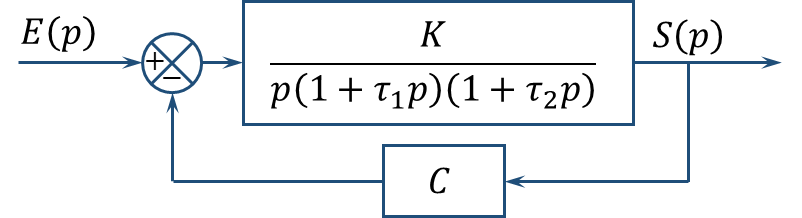
\includegraphics[width=.9\linewidth]{501_01}
\end{center}
 \fi
 
\question{Déterminer la valeur finale de $s(t)$ lorsque l'entrée est un échelon d'amplitude $E_0$.}
\ifprof
On a 
$H(p)=\dfrac{\dfrac{K}{p\left(1+\tau_1 p \right)\left(1+\tau_2 p \right)}}{1+\dfrac{CK}{p\left(1+\tau_1 p \right)\left(1+\tau_2 p \right)}}$
$=\dfrac{K}{p\left(1+\tau_1 p \right)\left(1+\tau_2 p \right)+CK}$. 
En conséquence, $S(p)=E(p)\dfrac{K}{p\left(1+\tau_1 p \right)\left(1+\tau_2 p \right)+CK}$.

$s_{\infty}=\lim\limits_{t\to +\infty} s(t)$ $=\lim\limits_{p\to 0} pS(p)$
$=\lim\limits_{p\to 0} pE(p)H(p)$.
Dans le cas où $E(p)$ est un échelon, on a $E(p)=\dfrac{E_0}{p}$ et donc 
$s_{\infty}=\lim\limits_{p\to 0} p\dfrac{E_0}{p}\dfrac{K}{p\left(1+\tau_1 p \right)\left(1+\tau_2 p \right)+CK}=\dfrac{E_0}{C}$.
\else 
\fi

%\question{En déduire la valeur de l'erreur statique.}
%\ifprof
%L'erreur statique est donnée par $\lim\limits_{t\to +\infty} (e(t)-s(t))=E_0 - \dfrac{E_0}{C}$.
%\else
%\fi

\question{Déterminer la valeur finale de $s(t)$ lorsque l'entrée est une rampe de pente $k$.}
\ifprof
On a maintenant $E(p)=\dfrac{k}{p^2}$. 
On a donc et donc 
$s_{\infty}=\lim\limits_{p\to 0} p\dfrac{k}{p^2}\dfrac{K}{p\left(1+\tau_1 p \right)\left(1+\tau_2 p \right)+CK}$ et 
$s_{\infty}=\infty$.

\else 
\fi


%\question{En déduire la valeur de l'erreur de traînage.}
%\ifprof
%$\varepsilon_v = \lim\limits_{t\to +\infty} (e(t)-s(t))$
%$=\lim\limits_{p\to 0} p\left(\dfrac{k}{p^2}-\dfrac{k}{p^2}\dfrac{K}{p\left(1+\tau_1 p \right)\left(1+\tau_2 p \right)+CK}\right)$
%
%$=\lim\limits_{p\to 0} \dfrac{k}{p}\left(1-\dfrac{K}{p\left(1+\tau_1 p \right)\left(1+\tau_2 p \right)+CK}\right)$
%$=\lim\limits_{p\to 0} \dfrac{k}{p}\dfrac{p\left(1+\tau_1 p \right)\left(1+\tau_2 p \right)+CK-K}{p\left(1+\tau_1 p \right)\left(1+\tau_2 p \right)+CK}=+\infty$
%\else
%\fi
%
%\question{Qu'en est-il si $C=1$ ?.}
%\ifprof
%$\varepsilon_v =\lim\limits_{p\to 0} \dfrac{k}{p}\dfrac{p\left(1+\tau_1 p \right)\left(1+\tau_2 p \right)+CK-K}{p\left(1+\tau_1 p \right)\left(1+\tau_2 p \right)+CK}$
%$=\lim\limits_{p\to 0} \dfrac{k}{p}\dfrac{p\left(1+\tau_1 p \right)\left(1+\tau_2 p \right)}{p\left(1+\tau_1 p \right)\left(1+\tau_2 p \right)+K}$
%$=\lim\limits_{p\to 0} k\dfrac{\left(1+\tau_1 p \right)\left(1+\tau_2 p \right)}{p\left(1+\tau_1 p \right)\left(1+\tau_2 p \right)+K} = \dfrac{k}{K}$.


%
%\else
%\fi
%\question{Réaliser le schéma-blocs.}
%\ifprof
%\begin{figure}[H]
%\centering
%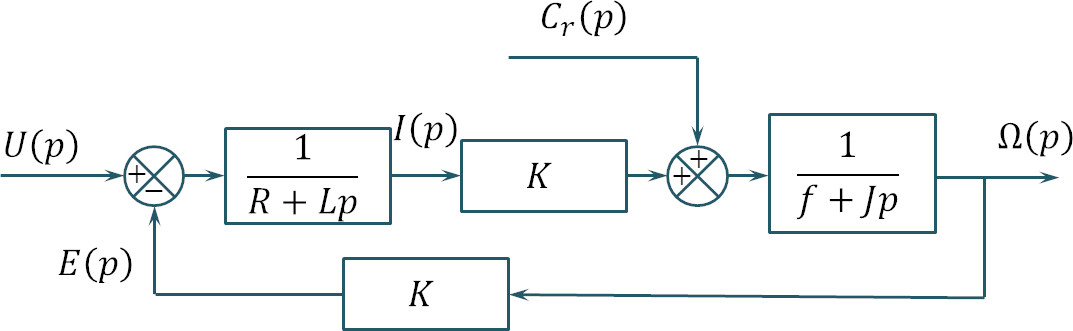
\includegraphics[width=\linewidth]{51_01_c}
%%\caption{Évolution du couple utile en fonction de la vitesse de rotation pour des
%%fréquences de commande de \SI{90}{Hz} à \SI{110}{Hz}. \label{fig_50_04}}
%\end{figure}
%\else
%\fi


 

\ifprof
\else

\noindent\footnotesize
\fbox{\parbox{.9\linewidth}{
Éléments de corrigé : 
\begin{enumerate}
    \item $s_{\infty}=\lim\limits_{p\to 0} p\dfrac{E_0}{p}\dfrac{K}{p\left(1+\tau_1 p \right)\left(1+\tau_2 p \right)+CK}=\dfrac{E_0}{C}$.
   % \item $\lim\limits_{t\to +\infty} (e(t)-s(t))=E_0 - \dfrac{E_0}{C}$.
    \item $s_{\infty}=\infty$.
   % \item $\varepsilon_v =\infty$.
%    \item $\varepsilon_v =\dfrac{k}{K}$.
\end{enumerate}}}
\normalsize

\begin{flushright}
\footnotesize{Corrigé  voir \ref{C2:03:501}.}
\end{flushright}%
\fi